\documentclass[aspectratio=169]{beamer}
\usetheme{Madrid}
\usecolortheme{default}
\usepackage{graphicx}
\usepackage{booktabs}
\title{Decision Tree Contribution}
\author{Ilaha Gadirli}
\date{}
\begin{document}

\begin{frame}{Decision Tree built from scratch}
\begin{columns}[T]
\begin{column}{0.48\textwidth}
\begin{itemize}
\item NumPy tree for log-price regression and premium/standard classification.
\item Sort each feature; test midpoints of adjacent distinct values.
\item Maximize impurity decrease: MSE, Gini, or entropy.
\item Four growth controls: depth, split size, leaf size, and minimum gain.
\item Leaf output: mean target or class frequencies.
\end{itemize}
\end{column}
\begin{column}{0.52\textwidth}
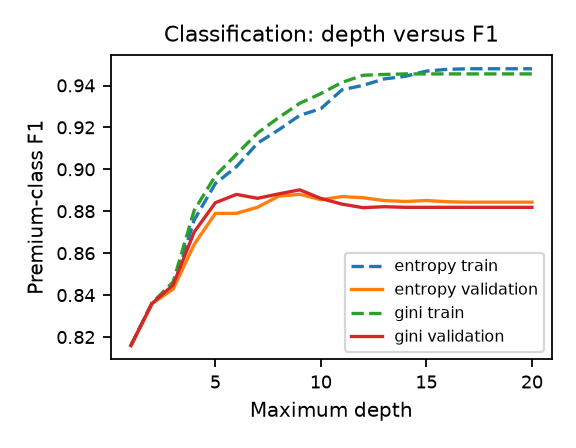
\includegraphics[width=\linewidth]{../report/figures/tree_classification_depth.png}
\end{column}
\end{columns}
\vspace{0.3em}
\small Validation selected Gini, depth 9, and at least 1 sample per leaf.
\end{frame}

\begin{frame}{Tree results and failure modes}
\small
\begin{tabular}{@{}lrr@{}}
\toprule
Held-out metric & Our tree & Matched sklearn tree \\
\midrule
Price RMSE (AZN) & 391{,}531 & 391{,}531 \\
Price MAE (AZN) & 99{,}840 & 99{,}840 \\
Tier F1 & 0.8952 & 0.8956 \\
Tier ROC-AUC & 0.9251 & 0.9246 \\
\bottomrule
\end{tabular}
\vspace{0.8em}

\begin{itemize}
\item Same 5{,}000 train rows; validation and test use full splits (9{,}406 each).
\item Tier errors: 35.9\% near the 212{,}000 AZN boundary, versus 10.6\% overall.
\item Price MAE: 547{,}009 AZN for luxury listings; 663{,}872 AZN for land plots.
\end{itemize}
\vspace{0.4em}
\footnotesize This is a single held-out split. The team benchmark supplies cross-validation uncertainty.
\end{frame}

\end{document}
